\documentclass[handout,aspectratio=169]{beamer}
\usetheme{default}

\usepackage{tikz}

\usepackage{amsmath,amssymb}

\newcommand{\pitem}{\pause\item}

\newtheorem{statement}{Statement}

\newcommand{\bits}{\{0,1\}}
\newcommand{\bitstr}{\bits^*}
\newcommand{\sshalf}{{\textstyle\frac12}}
\newcommand{\seqn}[2]{{#1}_1,{#1}_2,\dotsc,{#1}_{#2}}
\newcommand{\seqin}[3]{{#1}_{{#2}_1},{#1}_{{#2}_2},\dotsc,{#1}_{{#2}_{#3}}}
\newcommand{\IC}{\mathrm{IC}}
\newcommand{\poly}{\mathrm{poly}}
\newcommand{\Nat}{\mathbb{N}}

\DeclareMathOperator{\dom}{dom}
\DeclareMathOperator{\rank}{rank}
\DeclareMathOperator{\rng}{rng}
\DeclareMathOperator*{\E}{\mathbb{E}}

\newenvironment{sol}{%
    \begin{block}{}%
        \setbeamercolor{block body}{bg=lightgray}%
    }{
\end{block}}

\AtBeginSection[]{
    \begin{frame}
        \vfill
        \centering
        \begin{beamercolorbox}[sep=8pt,center,shadow=true,rounded=true]{title}
            \usebeamerfont{title}\insertsectionhead\par%
        \end{beamercolorbox}
        \vfill
    \end{frame}
}


\title{Property of Distributions}
\author{Alexander Smal at NUP}
\date{30.10.2024.\\ Lecture 4}

\begin{document}
    %%%%%%%%%%%%%%%%%%%%%%%%%%%%%%%%%%%%%%%%%%%%%%%%%%%%%%%%%%%%%%%%%%%%%%%%
    \begin{frame}[plain]
        \maketitle
    \end{frame}
    %%%%%%%%%%%%%%%%%%%%%%%%%%%%%%%%%%%%%%%%%%%%%%%%%%%%%%%%%%%%%%%%%%%%%%%%

    \section{Entropy Profiles}
    %%%%%%%%%%%%%%%%%%%%%%%%%%%%%%%%%%%%%%%%%%%%%%%%%%%%%%%%%%%%%%%%%%%%%%%%
    \begin{frame}{One variable}
		\begin{statement}
		    For any \(h \ge 0\), there exists a distribution \(\alpha\) such that \(H(\alpha) = h\).
		\end{statement}
		\pause
		\begin{proof}
		    Take some integer \(n\): \(0 \le h \le \log n\). The desired distribution is a linear combination of the distributions with probabilities \((1, 0, \dotsc, 0)\) and \((\frac{1}{n}, \frac{1}{n}, \dotsc, \frac{1}{n})\).
		\end{proof}
    \end{frame}
    %%%%%%%%%%%%%%%%%%%%%%%%%%%%%%%%%%%%%%%%%%%%%%%%%%%%%%%%%%%%%%%%%%%%%%%%

    %%%%%%%%%%%%%%%%%%%%%%%%%%%%%%%%%%%%%%%%%%%%%%%%%%%%%%%%%%%%%%%%%%%%%%%%
    \begin{frame}{Two variables}
		Let's consider the \emph{entropy profile} \((H(\alpha), H(\beta), H(\alpha, \beta))\).
		\begin{statement}
		    For any numbers \(h_1, h_2, h_{12} \ge 0\) that satisfy the following relations:
		\[
		    \left\{
		    \begin{array}{lll}
		        h_{12} \le h_1 + h_2 & \iff & t_0 = I(\alpha:\beta) \ge 0,\\
		        h_{2} \le h_{12}     & \iff & t_1 = H(\alpha \mid \beta) \ge 0,\\
		        h_{1} \le h_{12}     & \iff & t_2 = H(\beta \mid \alpha) \ge 0.
		    \end{array}
		    \right.
		\]
		    there exists a pair of random variables \((\alpha, \beta)\) with the entropy profile \((h_1, h_2, h_{12})\).
		\end{statement}
    \end{frame}
    %%%%%%%%%%%%%%%%%%%%%%%%%%%%%%%%%%%%%%%%%%%%%%%%%%%%%%%%%%%%%%%%%%%%%%%%

    %%%%%%%%%%%%%%%%%%%%%%%%%%%%%%%%%%%%%%%%%%%%%%%%%%%%%%%%%%%%%%%%%%%%%%%%
    \begin{frame}{Two variables (proof)}
		\begin{proof}
		    Let \(\xi_0, \xi_1, \xi_2\) be independent random variables with entropies \(t_0, t_1, t_2\) respectively. Then \(\alpha = (\xi_0, \xi_1)\) and \(\beta = (\xi_0, \xi_2)\) will be the desired variables.\bigskip
		
		    \begin{center} \mbox{}\hfill
		    \parbox{.4\textwidth}{\centering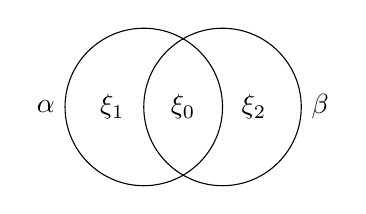
\begin{tikzpicture}
		    \tikzstyle{circ}=[circle, draw, inner sep=0pt, minimum width=2cm]
		
		    \node[circ, label=left:$\alpha$] (a) at (0,0) {};
		    \node[circ, label=right:$\beta$] (b) at (1,0) {};
		    \node at (-.4,0) {$\xi_1$};
		    \node at (1.4,0) {$\xi_2$};
		    \node at (.5,0)  {$\xi_0$};
		    \end{tikzpicture}}\hfill
		    	\parbox{.5\textwidth}{
		            \[
		            \begin{cases}
		                H(\xi_0) = t_0 = h_1 + h_2 - h_{12},\\
		                H(\xi_1) = t_1 = h_{12} - h_{2},\\
		                H(\xi_2) = t_2 = h_{12} - h_{1}.\\
		            \end{cases}
		            \]\qedhere}
		    \end{center}
		\end{proof}
    \end{frame}
    %%%%%%%%%%%%%%%%%%%%%%%%%%%%%%%%%%%%%%%%%%%%%%%%%%%%%%%%%%%%%%%%%%%%%%%%

    %%%%%%%%%%%%%%%%%%%%%%%%%%%%%%%%%%%%%%%%%%%%%%%%%%%%%%%%%%%%%%%%%%%%%%%%
    \begin{frame}{Three variables}
		The entropy profile for the triplet \((\alpha, \beta, \gamma)\) will be defined by 7 numbers:
		\[
		\bigl(H(\alpha), H(\beta), H(\gamma), H(\alpha, \beta), H(\alpha, \gamma),
		H(\beta, \gamma), H(\alpha, \beta, \gamma)\bigr).
		\]
		For the random variables \((\alpha, \beta, \gamma)\), we can write 9 independent inequalities.
		\begin{equation*}
		\begin{array}{lll}
		H(\alpha \mid \beta, \gamma) \ge 0, & I(\alpha : \beta) \ge 0, & I(\alpha : \beta \mid \gamma) \ge 0,\\
		H(\beta \mid \gamma, \alpha) \ge 0, & I(\beta : \gamma) \ge 0, & I(\beta : \gamma \mid \alpha) \ge 0,\\
		H(\gamma \mid \alpha, \beta) \ge 0, & I(\gamma : \alpha) \ge 0, & I(\gamma : \alpha \mid \beta) \ge 0.
		\end{array}
		\end{equation*}
		\begin{definition}
		Define the mutual information of three random variables as
		\[
		    I(\alpha : \beta : \gamma) = I(\alpha : \beta) - I(\alpha : \beta \mid \gamma).
		\]
		\end{definition}
    \end{frame}
    %%%%%%%%%%%%%%%%%%%%%%%%%%%%%%%%%%%%%%%%%%%%%%%%%%%%%%%%%%%%%%%%%%%%%%%%

    %%%%%%%%%%%%%%%%%%%%%%%%%%%%%%%%%%%%%%%%%%%%%%%%%%%%%%%%%%%%%%%%%%%%%%%%
    \begin{frame}{Three variables: geometric interpretation}
	    \begin{center}
	    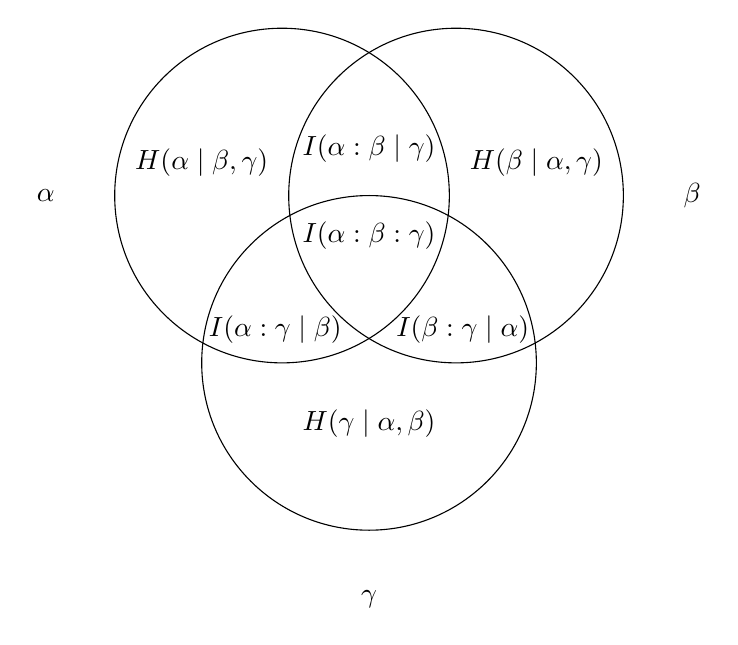
\begin{tikzpicture}[scale=0.85]
	        \tikzstyle{circ}=[circle, draw, inner sep=0pt, minimum width=5cm]
	
	        \draw(1.2,2) circle(2.5cm) node[xshift=-3cm]{$\alpha$};
	        \draw(3.8,2) circle(2.5cm) node[xshift=3cm] {$\beta$};
	        \draw(2.5,-0.5) circle(2.5cm) node[yshift=-3cm] {$\gamma$};
	
	        \node at (0,2.5) {$H(\alpha \mid \beta, \gamma)$};
	        \node at (5,2.5) {$H(\beta \mid \alpha, \gamma)$};
	        \node at (2.5,-1.4) {$H(\gamma \mid \alpha, \beta)$};
	
	        \node at (1.1,0) {$I(\alpha : \gamma \mid \beta)$};
	        \node at (2.5,2.7) {$I(\alpha : \beta \mid \gamma)$};
	        \node at (3.9,0) {$I(\beta : \gamma \mid \alpha)$};
	
	        \node at (2.5,1.4) {$I(\alpha : \beta : \gamma)$};
	    \end{tikzpicture}
	    \end{center}
    \end{frame}
    %%%%%%%%%%%%%%%%%%%%%%%%%%%%%%%%%%%%%%%%%%%%%%%%%%%%%%%%%%%%%%%%%%%%%%%%

    %%%%%%%%%%%%%%%%%%%%%%%%%%%%%%%%%%%%%%%%%%%%%%%%%%%%%%%%%%%%%%%%%%%%%%%%
    \begin{frame}{Three variables: properties}
		\begin{statement}
		    $I(\alpha:\beta:\gamma)$ can be negative.
		\end{statement}
		\begin{statement}
		    There are no other inequalities for triples.
		\end{statement}
		\begin{statement}
		    The measure of profiles that cannot be realized by any distribution is 0.
		\end{statement}
	\end{frame}
    %%%%%%%%%%%%%%%%%%%%%%%%%%%%%%%%%%%%%%%%%%%%%%%%%%%%%%%%%%%%%%%%%%%%%%%%

    %%%%%%%%%%%%%%%%%%%%%%%%%%%%%%%%%%%%%%%%%%%%%%%%%%%%%%%%%%%%%%%%%%%%%%%%
    \begin{frame}{Shearer's inequality}
		\begin{statement}
		    \(2H(\alpha, \beta, \gamma) \le H(\alpha, \beta) + H(\alpha, \gamma) + H(\beta, \gamma)\).
		\end{statement}
		\begin{theorem}[Shearer's Lemma]
		    Let \(X\) be a random variable distributed over \(\bits^n\).
		    For any distribution \(S\) on subsets of \([n]\), where
		    \(\Pr[i \in S] \ge \mu\), it holds that \(\E[H(X_S)] \ge \mu \cdot H(X)\).
		\end{theorem}

    \end{frame}
    %%%%%%%%%%%%%%%%%%%%%%%%%%%%%%%%%%%%%%%%%%%%%%%%%%%%%%%%%%%%%%%%%%%%%%%%

    %%%%%%%%%%%%%%%%%%%%%%%%%%%%%%%%%%%%%%%%%%%%%%%%%%%%%%%%%%%%%%%%%%%%%%%%
    \begin{frame}{Shearer's inequality: Counting Triangles in a Graph}
		    Let \(G = (V, E)\) be an undirected graph with \(t\) triangles, and let \(\ell = |E|\).\\
		    Let's show that \(t \le \frac{(2\ell)^{3/2}}{6}\).
		    \pause \begin{proof}
		        Let the triplet of random variables \((\alpha, \beta, \gamma)\) be uniformly distributed over the vertices of the triangles, and let \(X = (\alpha, \beta, \gamma)\). Then \(H(X) = H(\alpha, \beta, \gamma) = \log(6t)\), since each triangle occurs with six different permutations. Consider the distribution \(S\), uniform on subsets \(\{1, 2, 3\}\) of size 2. Then \(\Pr[i \in S] = \frac{2}{3}\). By Shirer's Lemma,
		    \[
		        \E_S[H(X_S)] \ge \frac{2}{3} \log(6t),
		    \]
		    i.e., there exists \(T \subset \{1, 2, 3\}\) for which \(H(X_T) \ge \frac{2}{3} \log(6t)\).
		    On the other hand, \(X_T\) is a distribution over the edges of the graph, so \(\log(2\ell) \ge H(X_T)\). From this, we get that \(2\ell \ge (6t)^{2/3}\).
		    \end{proof}

    \end{frame}

    %%%%%%%%%%%%%%%%%%%%%%%%%%%%%%%%%%%%%%%%%%%%%%%%%%%%%%%%%%%%%%%%%%%%%%%%
    \begin{frame}{Four variables and more}
		\begin{statement}[Inequality for 5 Random Variables]
		    $
		        I(a : b) \le I(a : b \mid x) + I(a : b \mid y) + I(x : y)
		        + I(a : b \mid z) + I(a : z \mid b) + I(b : z \mid a).
		    $
		\end{statement}
		\begin{corollary}[Zhang, Yeung, 1998]
		    An inequality for 4 random variables that cannot be expressed through the basic inequalities.
		    \[
		        I(a : b) \le 2I(a : b \mid x) + I(a : b \mid y) + I(x : y)
		        + I(a : x \mid b) + I(b : x \mid a).
		    \]
		\end{corollary}
		\begin{statement}
		    For 4 random variables, there are infinitely many inequalities that are independent of each other.
		\end{statement}
		
    \end{frame}
    %%%%%%%%%%%%%%%%%%%%%%%%%%%%%%%%%%%%%%%%%%%%%%%%%%%%%%%%%%%%%%%%%%%%%%%%

	\section{Inequalities for Triplets}
    %%%%%%%%%%%%%%%%%%%%%%%%%%%%%%%%%%%%%%%%%%%%%%%%%%%%%%%%%%%%%%%%%%%%%%%%
    \begin{frame}{Warm up}
		We will prove the following statement under various assumptions:
		\[
		    H(a \mid x) + H(a \mid y) \le H(a).
		\]
		
		\begin{problem}
		    If \(a, x, y\) are such that
		\[
		    \begin{cases}
		        H(a \mid x, y) = 0,\\
		        I(x : y \mid a) = 0.
		    \end{cases}
		\]
		then \(H(a \mid x) + H(a \mid y) \le H(a)\).
		\end{problem}
    \end{frame}
    %%%%%%%%%%%%%%%%%%%%%%%%%%%%%%%%%%%%%%%%%%%%%%%%%%%%%%%%%%%%%%%%%%%%%%%%

    %%%%%%%%%%%%%%%%%%%%%%%%%%%%%%%%%%%%%%%%%%%%%%%%%%%%%%%%%%%%%%%%%%%%%%%%
    \begin{frame}{Inequality for triplets}
    \begin{theorem}
        If \(a, x, y\) are such that \(H(a \mid x, y) = 0\) and
    \[
        \begin{cases}
            A_i \sim X_j\\
            A_i \sim Y_k
        \end{cases} \implies A_i \sim (X_j, Y_k),
    \]
    then \(H(a \mid x) + H(a \mid y) \le H(a)\).
    \end{theorem}

    \medskip (The notation \(A_i \sim X_j\) means \(\Pr[a = A_i \land x = X_j] > 0\).)
    \end{frame}
    %%%%%%%%%%%%%%%%%%%%%%%%%%%%%%%%%%%%%%%%%%%%%%%%%%%%%%%%%%%%%%%%%%%%%%%%

    %%%%%%%%%%%%%%%%%%%%%%%%%%%%%%%%%%%%%%%%%%%%%%%%%%%%%%%%%%%%%%%%%%%%%%%%
    \begin{frame}{Inequality for triplets: interpretation}
        Consider a bipartite graph with vertices \((L, R)\) with colored edges.
        All edges incident to a single vertex are of different colors, the degree in the left part is at least \(n\),
        and in the right part is at least \(m\). Suppose it is known that for a pair of vertices \((x \in L, y \in R)\)
        there is at most one common color. Prove that the number of colors is at least \(n \cdot m\).

        Note that monochrome edges form matchings. For each color \(c\), connect all
        vertices on the left that are matched with \(c\) to those on the right that are matched with \(c\). This forms a biclique of
        edges of color \(c\).

        Consider the distribution on triplets \((a, x, y)\) (color, vertex from the left part, vertex from the right
        part): we choose the color proportionally to the size (number of edges) of the corresponding biclique and
        select a random edge of that color. It can be checked that the following relation holds:
    \[
        \begin{cases}
            A_i \sim X_j,\\
            A_i \sim Y_k,
        \end{cases} \implies A_i \sim (X_j, Y_k).
    \]
    Now we apply: \(\underbrace{H(a \mid x)}_{\ge \log n} +
                      \underbrace{H(a \mid y)}_{\ge \log m} \le H(a) \le \log (\text{\# colors})\).
    \end{frame}
    %%%%%%%%%%%%%%%%%%%%%%%%%%%%%%%%%%%%%%%%%%%%%%%%%%%%%%%%%%%%%%%%%%%%%%%%

    %%%%%%%%%%%%%%%%%%%%%%%%%%%%%%%%%%%%%%%%%%%%%%%%%%%%%%%%%%%%%%%%%%%%%%%%
    \begin{frame}{Conditional Inequality for a Quadruples}
		\begin{statement}
		    If for random variables \(a, b, x, y\) the following holds
		    \[
		        \begin{cases}
		            I(x:y \mid a) = 0,\\
		            H(a \mid x, y) = 0,
		        \end{cases}
		    \]
		    then \(I(a:b) \le I(a:b \mid x) + I(a:b \mid y) + I(x:y)\).
		\end{statement}
    \end{frame}
    %%%%%%%%%%%%%%%%%%%%%%%%%%%%%%%%%%%%%%%%%%%%%%%%%%%%%%%%%%%%%%%%%%%%%%%%


\end{document}
